\documentclass{article}
\usepackage{listings}
\usepackage{pdfpages}
\graphicspath{ {.} }

\usepackage{fancyhdr}
\usepackage[pdftex,
	pdfauthor={Aryan Gupta},
	pdftitle={ECGR4181 HW1 Report},
	pdfsubject={Homework Report},
	pdfkeywords={},
	pdfproducer={Latex with hyperref},
	pdfcreator={}
]{hyperref}
\usepackage[margin=1in]{geometry}
\hypersetup{colorlinks=true, linkcolor=black,urlcolor=black}
\usepackage[margin=1in]{geometry}
\usepackage{lastpage}
\usepackage[margin=1in]{geometry}
\usepackage{fancyhdr}
\usepackage{amsmath,amsfonts, amsthm}
\usepackage{float}
\usepackage{graphicx}


\lstset{
  basicstyle=\ttfamily,
  columns=fullflexible,
  frame=single,
  breaklines=true,
  postbreak=\mbox{$\hookrightarrow$\space},
}

\begin{document}
	\section{Dinero Simulator}
		The Dinero simulator is a cache simulator that lets the use experiment with different cache options such as associativity and block size. We modified various options to determine how it affects the cache miss ratio. The 12 main options given to us to test out are listed below.
		\begin{itemize}
			\item Split cache with 8Byte blocks directally mapped
			\item Split cache with 8Byte blocks 4 way associative
			\item Split cache with 32Byte blocks directally mapped
			\item Split cache with 32Byte blocks 4 way associative
			\item Split cache with 128Byte blocks directally mapped
			\item Split cache with 128Byte blocks 4 way associative
			\item Unified cache with 8Byte blocks directally mapped
			\item Unified cache with 8Byte blocks 4 way associative
			\item Unified cache with 32Byte blocks directally mapped
			\item Unified cache with 32Byte blocks 4 way associative
			\item Unified cache with 128Byte blocks directally mapped
			\item Unified cache with 128Byte blocks 4 way associative
		\end{itemize}
		The split caches were comprised of 16KB instruction cache and 16KB data cache. The unified caches were 32KB large. These experiments were ran using this command for split cache.
		\begin{lstlisting}
cat ../../project/trace.din | ./dineroIV -l1-dsize <DATA_CACHE_SIZE> -l1-dbsize <DATA_BLOCK_SIZE> -l1-dassoc <DATA_ASSOC> -l1-isize <INS_CACHE_SIZE> -l1-ibsize <INS_BLOCK_SIZE> -l1-iassoc <INS_ASSOC> -informatd
		\end{lstlisting}
		And this command for unified cache.
		\begin{lstlisting}
cat ../../project/trace.din | ./dineroIV -l1-usize <CACHE_SIZE> -l1-ubsize <BLOCK_SIZE> -l1-uassoc <DATA_ASSOC> -informatd
		\end{lstlisting}
		\par
		The result of the experiment with the dineroIV simulator was consistant with the theroy tought in class. The results are laied neatly in this graoh below.
		\begin{figure}[H]
			\centering
			\label{fig:uniMetric}
			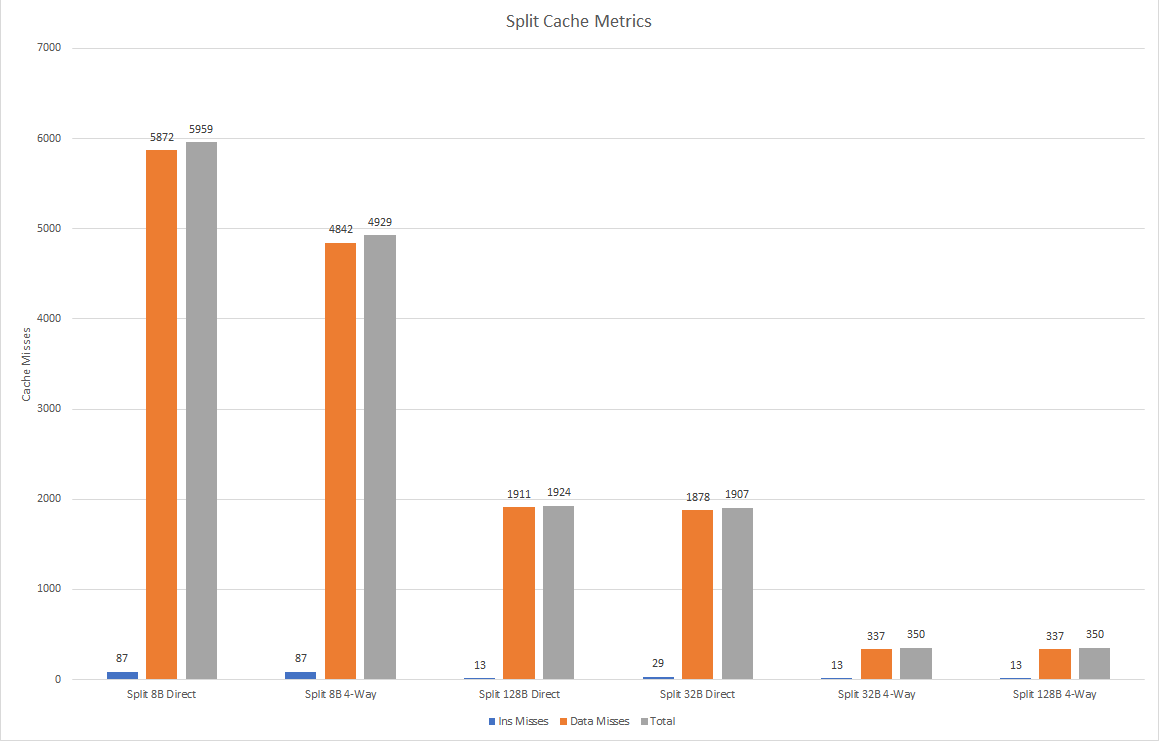
\includegraphics[width=\textwidth]{uni-cache-metrics.png}
			\caption{Metrics of a unified cache}
		\end{figure}
		A general trend that can be seen in Figure \ref{fig:uniMetric} is that as the associativity increases the miss rate drops. This is because when the associativity is increased a cache line is less likely to fight another line for a spot in the cache. This type of cache miss is known as conflict misses because 2 lines are confilicting for a spot in the cache. Another trend that can be seen is that as the size of the cache line is increased, the miss rate drops. This is because as the cache line size is increased the spacial locality of that line is also increased. When data is accessed, it is highly likly that some data next to or around that data will be accessed next or in the near future. By increasing the blick size, we can take advantage of this fact and load possible future memory access into the cache befoire they are actually accessed. This type of cache is usually used in L2 caches because the data and instructions dont need to be seperated.
		\par
		Contrary to the L2 cache, the L1 cache is usually split by the data and instructions. This means that there are 2 "caches", one for the instructions and another one for data. This can benefit drastically because the way instructions are accessed is very different from the way data is accessed. Instructions have alor more spatial locaity and Data have more temporoal locality. Figure \ref{fig:splitMetric} is a graph representing the metrics of the split cache.
		\begin{figure}[H]
			\label{fig:splitMetric}
			\begin{center}
				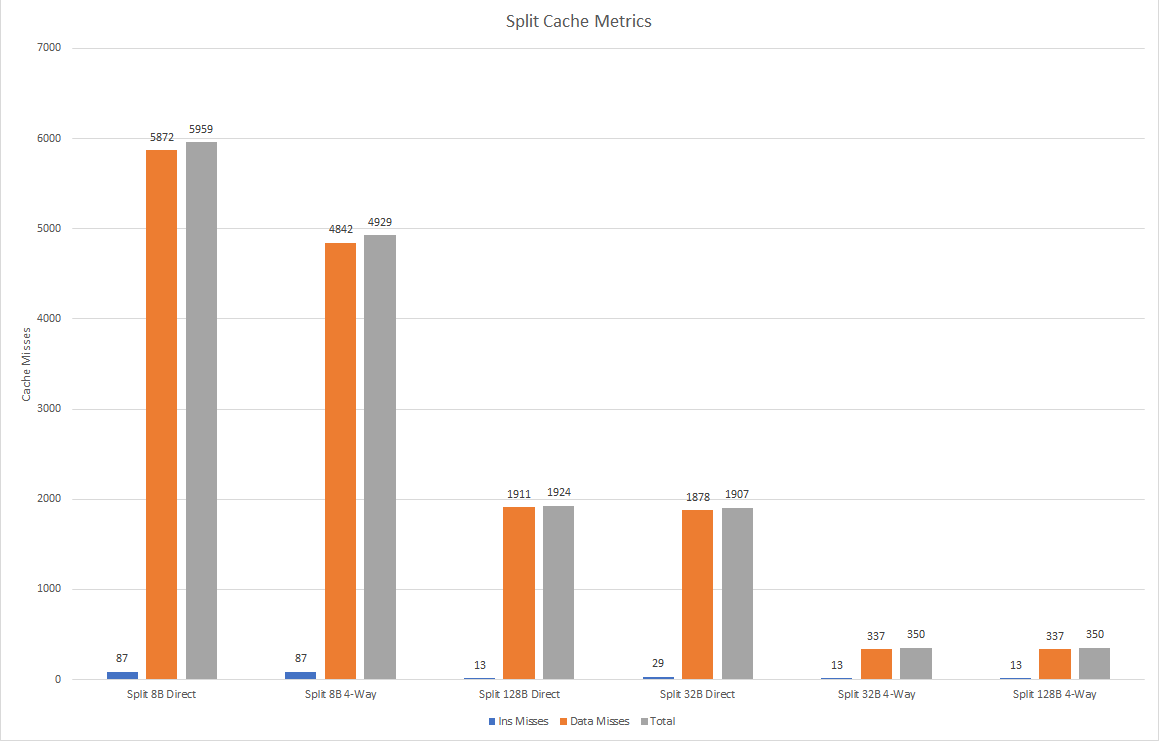
\includegraphics[width=\textwidth]{spl-cache-metrics.png}
				\caption{Metrics of a unified cache}
			\end{center}
		\end{figure}
		The graph plainly represents a decrease in cache misses as the associativity and cache block sizes are increased. These results are inline with the theory learned in class.
		\par
		Figure \ref{fig:diffMetric} shows the differece betweek using a split cache and a unified cache. There does not seem to be any clear pattern between using a split or unified cache. More experimentation is needed before anything concrete can be deducted.
		\begin{figure}[H]
			\label{fig:diffMetric}
			\begin{center}
				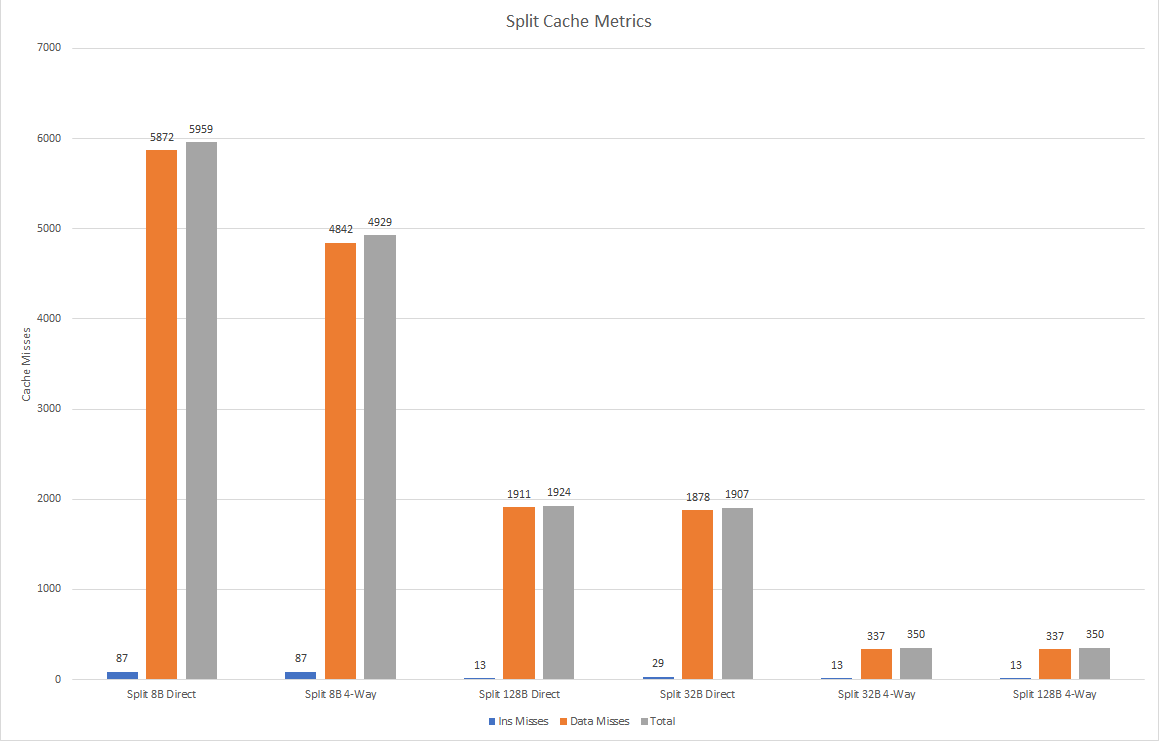
\includegraphics[width=\textwidth]{spl-cache-metrics.png}
				\caption{Metrics of a unified cache}
			\end{center}
		\end{figure}

	\subsection{Custom Cache Simulator}
		For part 2 of the assignment, we created our own Simulator similar to dineroIV. The code for this project is located in the \verb|src/| directory. I am using Arch Linux and I reconize that older systems may not support all the features used in the build system. I have tried as much as I could to add legacy support for older build systems. I was able to compile using gcc version 5 without any issues. In case you arent able to build the code, there is a prebuild binary in the \verb|bin/| directory named \verb|main.out|. To rebuild the binary, please run \verb|~$ make all| or just \verb|~$ make|.
		\subsubsection{The Code}
			The code consists of these classes
			\begin{itemize}
				\item Simulator
				\item Cache
				\item parse
				\item printer
			\end{itemize}
			The Simulator class is responsible for running the simulator. The c'tor of the class takes in a the instructions to execute and parsed data from the command line. Using this information, the Simulator sets up the hiearchy of cache and then begins executing the instructions at the call of \verb|Simulator::simulate()|. Another member function: \verb|Simulator::getRatio()| returns the ratio of hits to the total number of access.
			\par
			The Cache class is where all the magic happens. The Cache class holds the addresses of the data that is currently in the cache. Because of associativity and the various other simulator options, there is also a valid bit and a Least Recently Used (lru) number. These 3 data members are grouped into a c-style struct called \verb|cache-info|. The lru bits will be discussed in greater detail later. Upon the construction of the Cache class, anotehr c-style struct is created that defines which parts of the address are the tag, index, or offset. This simplifies the extraction of these bits during computation. An example is shown below.
			\begin{center}
			\begin{verbatim}
                        0x25F287AB
                        0b10010111110010  100001111010  1011
                          ~~~~~~~~~~~~~~  ~~~~~~~~~~~~  ~~~~
                                Tag           Index    Offset
			\end{verbatim}
			\end{center}
			In this example, the block-size is 16B and the Cache is 64KB. The offset bits are easy and can be calculated by using this equation.
			\[ Offset Bits = log_2(blocksize) = log_2(16) = 4  \]
			The Index bits can be calcuated by taking the cache size (64KB) and dividing it by the block-size.
			\[ Index Bits = log_2\left(\frac{cachesize}{blocksize}\right) = log_2\left(\frac{64KB}{16B}\right) = log_2\left(\frac{65536}{16}\right) = 12 \]
			The rest of the 32 bits are the tag.
			\[ Tag bits = 32 - blockbits - cachesize = 32 - 4 - 12 = 16 \]
			Using these 3 pieces of information, the masks and bit shifts can be calaculated to extract each part of the address. More details can be viewed in \verb|Cache::getTag(ptr_t)|. Once the cache sizes and address bits are set, the replace and locate function are computed.


	\subsection{Pintools}


\end{document}